% English-language manuscript for the MDPI journal Vehicles.
\documentclass[vehicles,article,submit,moreauthors]{Definitions/mdpi}

\firstpage{1}
\makeatletter
\setcounter{page}{\@firstpage}
\makeatother
\pubvolume{1}
\issuenum{1}
\articlenumber{0}
\pubyear{2026}
\copyrightyear{2026}
\datereceived{ }
\daterevised{ }
\dateaccepted{ }
\datepublished{ }

\Title{Field Telemetry and Route Characterization of a Solar-Assisted Light Electric Vehicle: Data-Quality Assessment and Measurement Requirements}

\newcommand{\orcidauthorA}{0009-0001-0880-1457}
\newcommand{\orcidauthorB}{0000-0003-4243-0597}
\newcommand{\orcidauthorC}{0009-0007-1592-5160}
\newcommand{\orcidauthorD}{0000-0002-8454-3306}
\Author{Santiago Pérez $^{1}$\orcidA{}, Paola Portero $^{1}$\orcidB{}, Carlos Cuaical $^{2}$\orcidC{}, and Maxwell Salazar $^{3,*}$\orcidD{}}
\AuthorNames{Santiago Pérez, Paola Portero, Carlos Cuaical, and Maxwell Salazar}
\address{%
$^{1}$ \quad Electrical Management and Maintenance Department, Instituto Tecnológico Superior Rumiñahui (ISTER), Sangolquí 171103, Ecuador\\
$^{2}$ \quad Systems and Data Management Department, Instituto Tecnológico Superior Rumiñahui (ISTER), Sangolquí 171103, Ecuador\\
$^{3}$ \quad Electronics Department, Instituto Tecnológico Superior Rumiñahui (ISTER), Sangolquí 171103, Ecuador}
\corres{Correspondence: maxwell.salazar@ister.edu.ec}

\abstract{Light electric vehicle prototypes with vehicle-integrated photovoltaics are often evaluated using low-cost telemetry whose measurement chain is rarely documented. This study characterizes field use and audits the telemetry of a single-seat prototype equipped with a 200 Wp photovoltaic array, a 2 kW brushless DC (BLDC) motor, and a 48 V gel-battery bank in Sangolquí, Ecuador (approximately 2500 m above sea level). Of 4277 GPS and electrical records collected in July and August 2026, 3052 records from 11 dates were retained. Eight sessions with at least 100 observations (3029 records) were summarized by session using a block bootstrap. The data revealed a repeatedly traveled route with an extent of approximately 1.4 km (mean speed, 14.7--16.0 km/h) and confined circuits with displacements below 0.15 km (7.7--8.7 km/h). The estimated speed matched the value derived from GPS coordinates (RMSE, 0.003 km/h); therefore, this comparison is not an independent validation. Motor current was bounded at $\pm 6.55$ A (6.9\% of observations), had a session-dependent baseline (mean values ranging from $+0.9$ to $-2.2$ A), and did not respond to speed ($R^2=0.003$) or acceleration ($\rho=-0.01$). The channel labeled as the panel current was bounded at $\pm 3.28$ A, with 34\% zero readings. The current measurement chain does not support estimates of energy consumption or photovoltaic generation; minimum instrumentation requirements are proposed.}

\keyword{light electric vehicle; vehicle-integrated photovoltaics; GPS telemetry; data quality; sensor saturation; field study}

\begin{document}

\section{Introduction}

Vehicle-integrated photovoltaics (VIPV) can turn vehicle surfaces into electricity generators and, in some configurations, supplement the energy stored in the battery. Reviews and modeling studies indicate that VIPV potential depends on active surface area, orientation, shading, temperature, irradiance, and usage patterns; therefore, design estimates cannot replace measurements made on the vehicle \citep{ref-commault,ref-sierra,ref-hoth,ref-kouzelis}. Field studies that quantify the output of vehicle-mounted modules require measurements of irradiance on the vehicle body and module temperature, together with a description of the driving profile \citep{ref-wetzel,ref-ng,ref-ota-irradiance,ref-ota-driving,ref-ota-curve}.

A growing body of research on light electric vehicles uses low-cost data loggers (GPS and voltage and current sensors) to describe real-world use and estimate energy consumption. These studies assume that each channel measures the quantity indicated by its label, with an adequate range and zero offset. However, the measurement chain is rarely documented, and common problems in field records (zero readings, spurious peaks, saturation, and zero drift) are addressed using filters that are seldom described in detail \citep{ref-bhavsar,ref-alwreikat}. Voltage- and current-sensor errors directly affect derived quantities \citep{ref-hu,ref-zheng}. Real-world driving cycles and GPS data analysis have been used to characterize the use of electric and light vehicles \citep{ref-pfriem,ref-brady,ref-uberti,ref-gurusamy}, but less attention has been paid to the validity of the accompanying electrical signals. Field data for solar-assisted light vehicles at equatorial latitudes and high elevations are also scarce, as is documentation of how telemetry signals from low-cost prototypes are assessed; both are relevant to vehicle development in the Andean region.

The analysis uses field records from a light electric vehicle prototype developed at the Instituto Tecnológico Superior Rumiñahui (ISTER) in Sangolquí, Ecuador, together with the vehicle's technical specifications. Specifically, it (i) characterizes GPS-tracked routes and speeds in an Andean setting, (ii) assesses whether the available electrical telemetry supports estimates of energy consumption or photovoltaic generation, and (iii) derives minimum measurement-chain requirements from the observed data-quality problems.
The vehicle's solar performance is not evaluated because the available data do not support such an assessment.

\section{Materials and Methods}

\subsection{Vehicle and Documented Specifications}

The prototype is a single-seat vehicle with a steel chassis, chain drive to the rear axle, and a mid-drive 48 V, 2 kW nominal BLDC motor. The motor's maximum design current is 46.3 A (57.9 A including the protection margin stated in the specifications). Two flexible BougeRV Arch100 modules (100 Wp, 100\,$\times$\,60 cm) connected in series form an array with $V_{\mathrm{mp}}=34.2$ V, $V_{\mathrm{oc}}=39.6$ V, and $I_{\mathrm{sc}}=6.16$ A. The array is connected to a 300 W DC HOUSE MPPT boost converter with an input range of 13--65 V. The energy-storage bank comprises four 12 V, 60 Ah gel batteries connected in series (valve-regulated lead-acid batteries with gelled electrolyte). The vehicle mass is not reported in the specifications. Figure~\ref{fig:prototipo} shows the overall configuration, and Figure~\ref{fig:unifilar} shows the single-line diagram with the recorded channels.

The same specifications include calculations of available power, efficiency, range, and design solar conditions (latitude $-0.31^\circ$; 5.08 peak-sun hours). These are documented specifications and were not used as experimental results: irradiance, module temperature, state of charge, and energy at the battery terminals were not measured.

\begin{figure}[H]
    \centering
    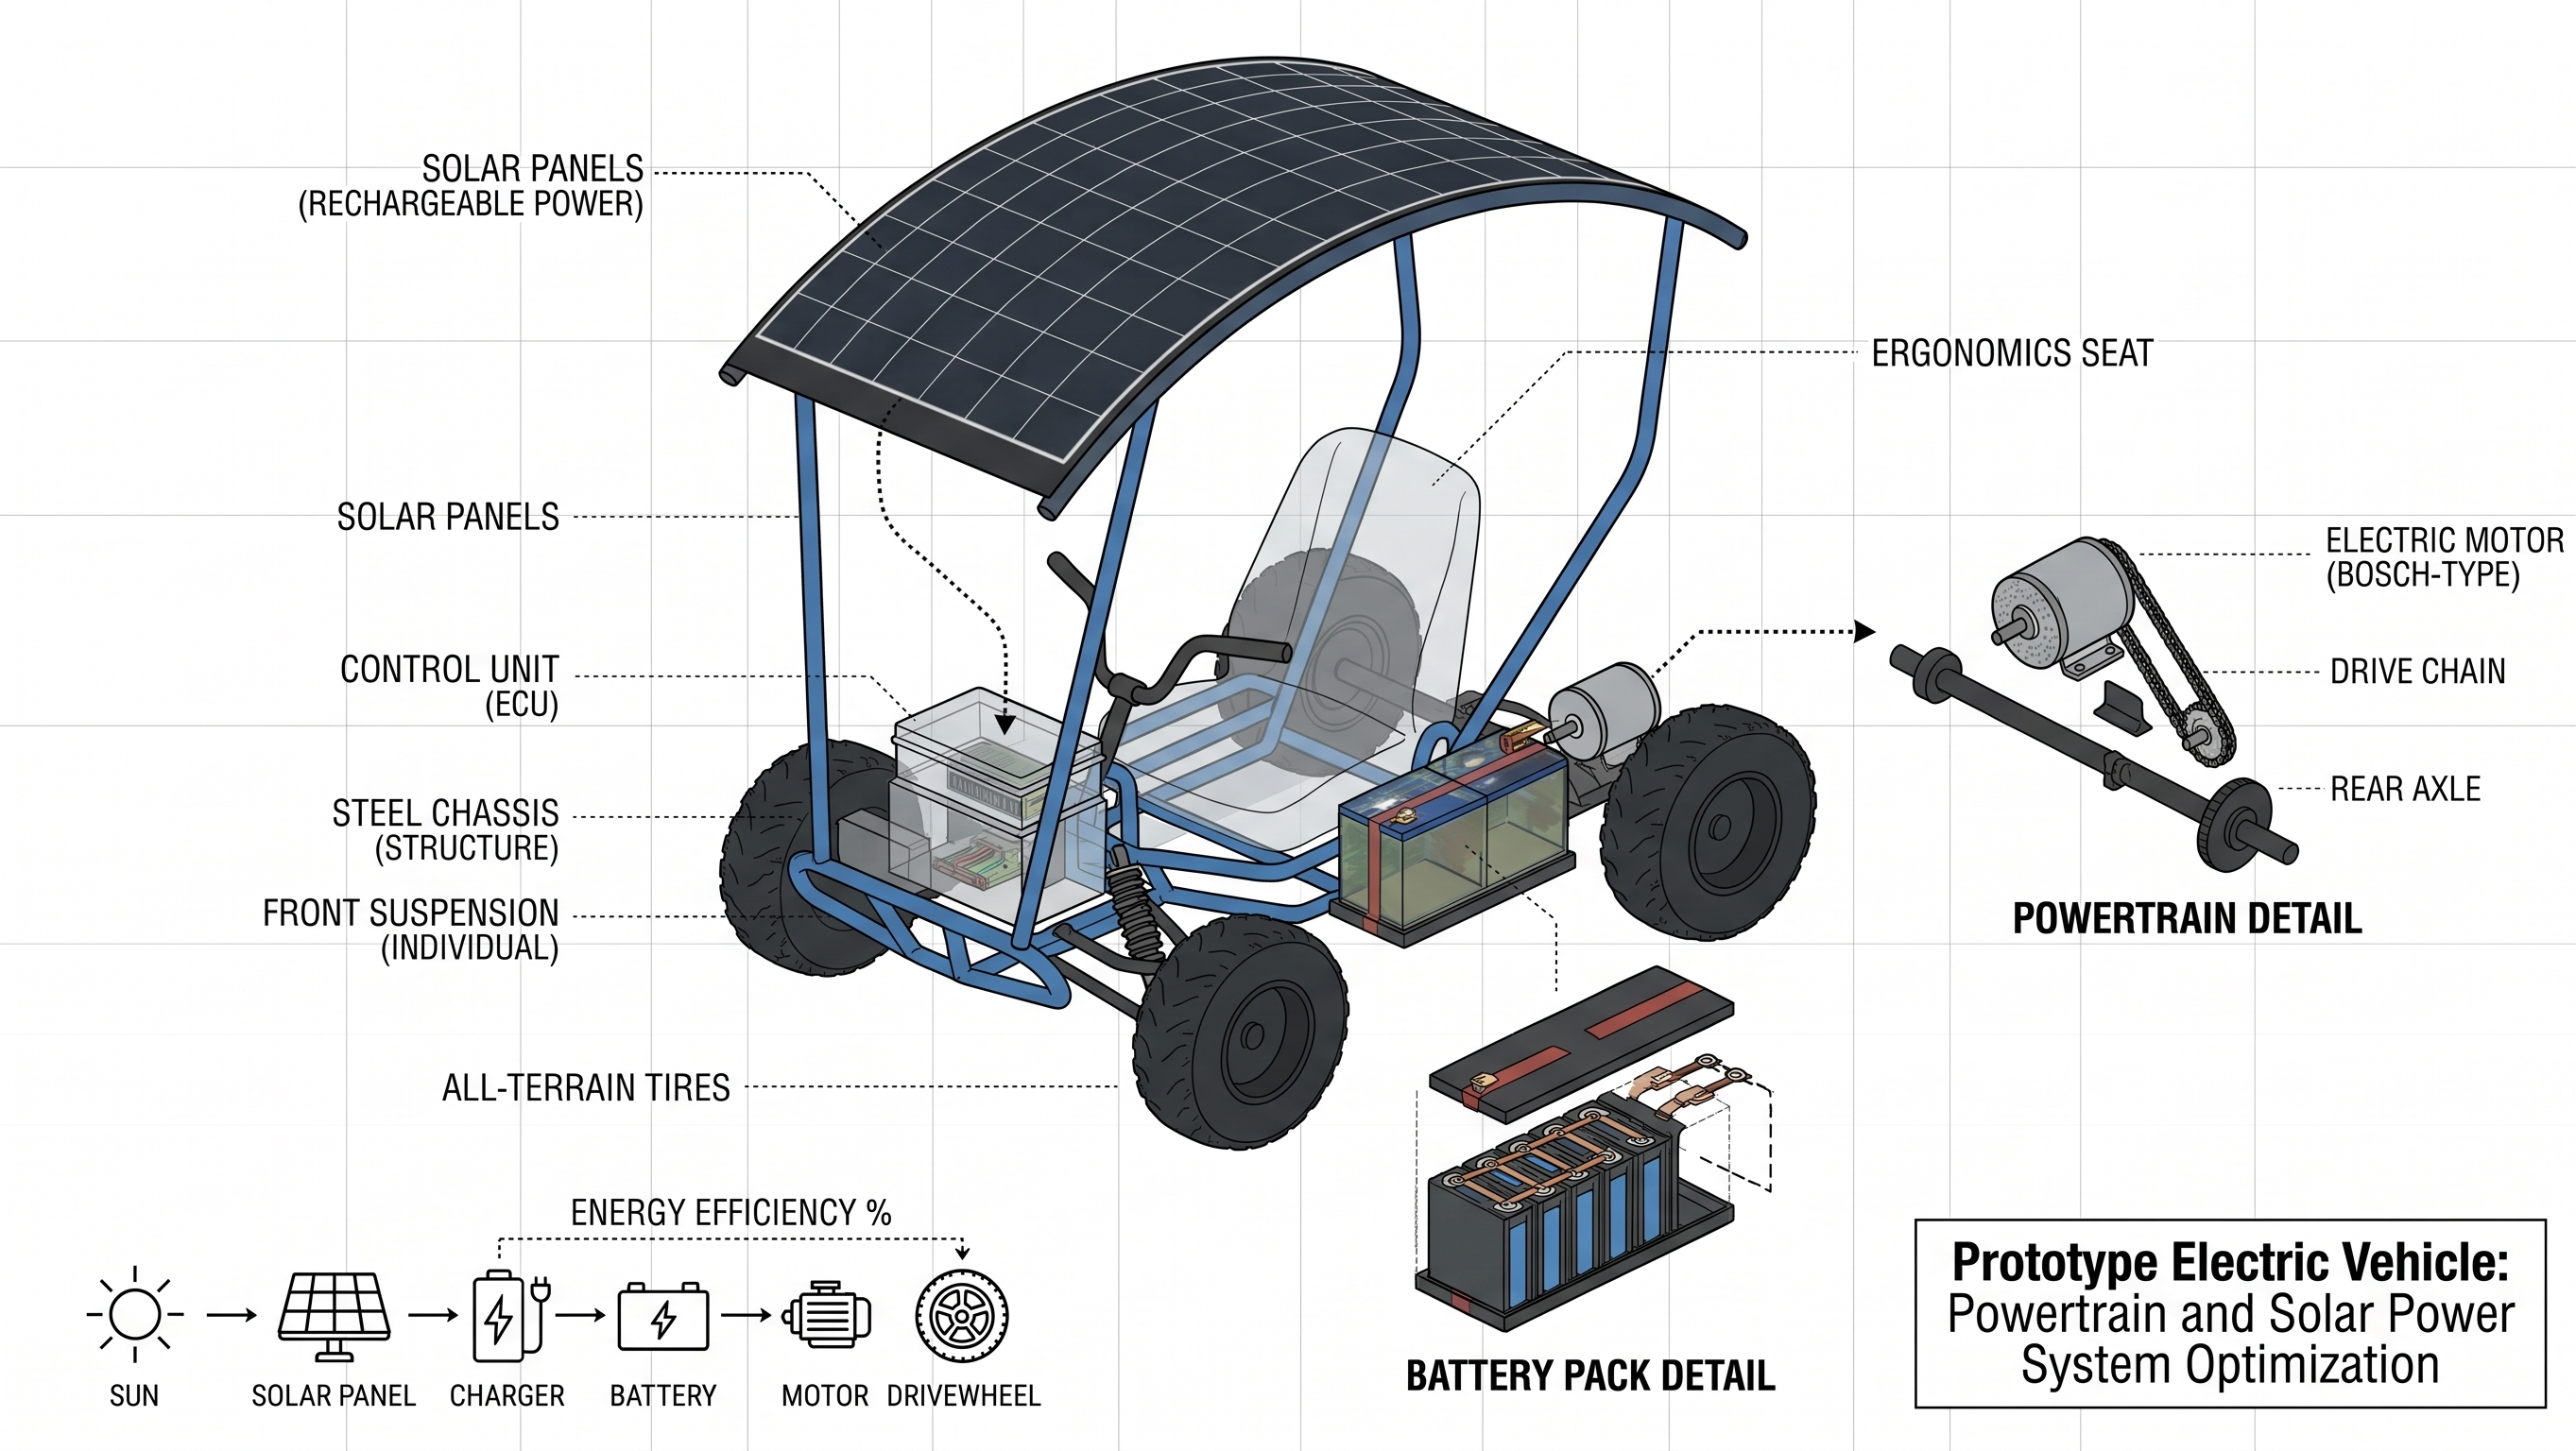
\includegraphics[width=\textwidth]{auto.jpg}
    \caption{Illustrative schematic of the prototype: roof-mounted flexible photovoltaic modules, control unit, steel chassis, battery bank, electric motor, chain drive, and rear axle. The figure is descriptive and does not represent measurements.\label{fig:prototipo}}
\end{figure}

\begin{figure}[H]
    \centering
    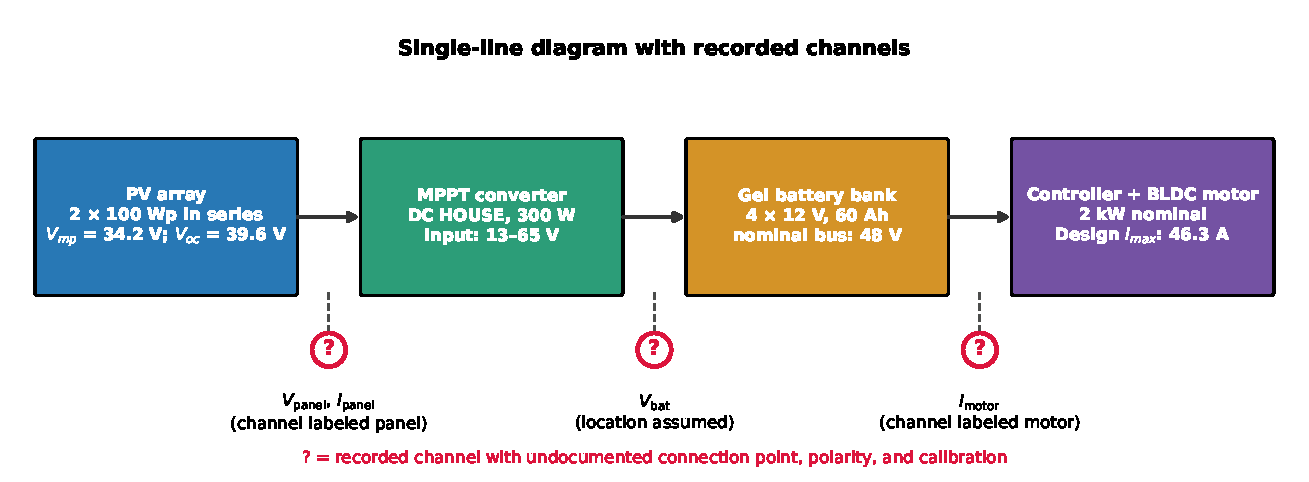
\includegraphics[width=\textwidth]{figuras/fig_2_unifilar_medidas}
    \caption{Single-line diagram of the system showing the telemetry channels. Nominal values are taken from the technical specifications. The connection points, polarity, and calibration of the voltage and current channels are undocumented (indicated by “?” symbols).\label{fig:unifilar}}
\end{figure}

\subsection{Data}

Two workbooks containing movement records (July and August 2026) and one consolidated workbook containing the retained data and the exclusion reason for each record were used. The movement workbooks contain 4277 records (3714 from July and 563 from August), previously filtered to estimated speeds between 1 and 120 km/h. The variables are timestamp (typically sampled every 5 s), battery voltage, voltage and current in channels labeled as panel and motor, GPS coordinates, distance increment, and estimated speed. The coordinates are not reproduced as georeferenced tracks; routes are shown in relative local coordinates.

The consolidated workbook retained 3052 records (71.4\%) across 11 dates and excluded 1225 (28.6\%) based on the following criteria: battery voltage outside 29.91--64.95 V or zero; panel voltage outside 4.46--54.73 V or zero; and panel current with $|I|>100$ A. Current signs were preserved. For between-session summaries, adequate coverage was defined as at least 100 observations on a date: eight dates (3029 records) met this criterion. The other three dates (1--18 records) are shown in Table~\ref{tab:sesiones} but are not included in between-session summaries. This threshold is an organizational criterion, not a test of data quality or representativeness; its effect is examined in the sensitivity analysis.

\subsection{Analysis}

\textbf{Movement summary.} Session-level summaries included the number of records, the sum of distance increments, mean and maximum speed, and dispersion statistics (median and interquartile range, IQR). The sum of increments is not necessarily the total distance traveled because prior movement-based filtering and excluded records leave gaps. Session geometry was summarized by the maximum displacement from the first point and the north--south and east--west extents in local coordinates.

\textbf{Speed consistency and driving profile.} The reported speed was compared with the speed derived from coordinates (Haversine distance between consecutive records divided by the time interval, for intervals of 4--6 s) using bias, Bland--Altman limits of agreement, and RMSE. Acceleration was calculated as the difference in reported speed between consecutive records (for intervals of 4--6 s). The speed--acceleration distribution and relative positive acceleration (RPA, $\sum v\,a^{+}\Delta t/\sum v\,\Delta t$) were calculated. Micro-trips were defined as segments of at least six records separated by gaps longer than 30 s. The relationship between acceleration and current was assessed using the Spearman coefficient for each session.

\textbf{Electrical signals.} Recorded electrical power was calculated as $P=V_{\mathrm{bat}}I_{\mathrm{motor}}$, preserving the channel sign, and integrated by session as $E=\sum P_i\Delta t_i$ over intervals of up to 30 s; the specific indicator is $E/d$. These quantities are termed signal indicators because sensor polarity, measurement point, and calibration are unknown. Current saturation (observations with $|I|\ge 6.55$ A and the duration of consecutive runs), the current baseline (session mean and mean at low speed), and the panel-channel distribution were quantified. The panel voltage was also compared with the array's $V_{\mathrm{mp}}$ and $V_{\mathrm{oc}}$, and its relationship with time of day was assessed. The relationship between speed and $|P|$ was summarized using linear regression with session-clustered errors (eight clusters, $t$ intervals with 7 degrees of freedom) and $R^2$. The empirical slope $R_{\mathrm{ef}}=-\Delta V_{\mathrm{bat}}/\Delta I_{\mathrm{motor}}$ was estimated using the same correction and session fixed effects; it represents an observed slope, not a measured internal resistance.

\textbf{Uncertainty and sensitivity.} Because consecutive observations are autocorrelated, session-level 95\% confidence intervals (CIs) were obtained using a moving-block bootstrap with blocks of 30 observations and 4000 resamples \citep{ref-kunsch}. Sensitivity was assessed to the minimum coverage threshold (50, 100, 200, and 400 records), the maximum integration interval (10, 30, 60, and 120 s), the minimum speed (1, 3, and 5 km/h), exclusion of saturated observations, and block length (15, 30, and 60). Between-month comparisons are described using medians and Cliff's $\delta$ \citep{ref-cliff}; no hypothesis tests were applied to autocorrelated observations. Calculations were performed in Python using SciPy and statsmodels \citep{ref-scipy,ref-statsmodels}, with a fixed random seed; the code is included in the project materials.

\section{Results}

\subsection{Coverage and Reasons for Exclusion}

The 4277 initial records were reduced to 3052 (Table~\ref{tab:exclusion}). The primary reason for exclusion was zero battery-voltage readings (46.7\% of exclusions), rather than outliers, followed by zero panel-voltage readings (40.9\%). A total of 35.6\% of excluded records failed more than one criterion, suggesting simultaneous acquisition losses. Four July dates (11, 13, 18, and 20) contributed only excluded records (247 in total). The proportion retained per date ranged from 2\% to 91\% (Supplementary Table S4). Coverage across retained dates was uneven: three dates had fewer than 100 records (21 July: 18; 23 July: 4; 1 August: 1).

\begin{table}[H]
    \caption{Reasons for exclusion of the 1225 discarded records. A record may fail more than one criterion.\label{tab:exclusion}}
    \small
    \begin{tabular}{l r r}
        \toprule
        \textbf{Failed criterion}                & \textbf{Records} & \textbf{\% of exclusions} \\
        \midrule
        Zero or invalid battery voltage          & 572              & 46.7                      \\
        Zero or invalid panel voltage            & 501              & 40.9                      \\
        Outlier battery voltage (MAD)            & 261              & 21.3                      \\
        Outlier panel voltage (MAD)              & 229              & 18.7                      \\
        Panel current out of range ($|I|>100$ A) & 102              & 8.3                       \\
        \midrule
        One / two / three criteria               & 789 / 432 / 4    & 64.4 / 35.3 / 0.3         \\
        \bottomrule
    \end{tabular}
    \begin{flushleft}
        \footnotesize MAD: median absolute deviation (threshold of 6 MAD from the median).
    \end{flushleft}
\end{table}

\subsection{Routes and Driving Profile}

The eight sessions with adequate coverage comprised two route types (Table~\ref{tab:sesiones}, Figure~\ref{fig:rutas}). From 27 to 31 July, a route with an approximately 1.4 km north--south extent was repeated, with maximum displacements of 1.24--1.25 km and recorded distances of 7.6--13.0 km. The 25 July session and the two August sessions followed confined circuits, with maximum displacements of 0.06--0.13 km. Session mean speed ranged from 14.7 to 16.0 km/h on the repeated route and from 7.7 to 8.7 km/h on the confined circuits (mean across the eight sessions, 12.54 $\pm$ 3.67 km/h; Supplementary Table S1). Median speed in July (13.99 km/h) was higher than in August (8.80 km/h; Cliff's $\delta=0.375$), but the difference coincides with route type and cannot be attributed to month.

\begin{table}[H]
    \caption{Movement metrics by date and route type.\label{tab:sesiones}}
    \small
    \setlength{\tabcolsep}{3pt}
    \begin{tabular}{l r r r r r l}
        \toprule
        \textbf{Date} & \textbf{Records} & \parbox{1.6cm}{\centering\textbf{Distance                                           \\(km)}} & \parbox{1.8cm}{\centering\textbf{Mean $v$\\(km/h)}} & \parbox{1.8cm}{\centering\textbf{Max. $v$\\(km/h)}} & \parbox{1.9cm}{\centering\textbf{Max.\\displ. (km)}} & \textbf{Type}\\
        \midrule
        21/07         & 18               & 0.080                                     & 3.18  & 11.10 & --   & (low coverage)   \\
        23/07         & 4                & 0.008                                     & 1.46  & 2.39  & --   & (low coverage)   \\
        25/07         & 114              & 1.226                                     & 7.74  & 16.87 & 0.10 & Confined circuit \\
        27/07         & 369              & 7.610                                     & 14.85 & 46.86 & 1.25 & Repeated route   \\
        28/07         & 448              & 9.966                                     & 16.02 & 49.23 & 1.25 & Repeated route   \\
        29/07         & 587              & 11.957                                    & 14.67 & 47.55 & 1.24 & Repeated route   \\
        30/07         & 638              & 13.009                                    & 14.68 & 43.08 & 1.24 & Repeated route   \\
        31/07         & 504              & 10.944                                    & 15.63 & 40.49 & 1.25 & Repeated route   \\
        01/08         & 1                & 0.002                                     & 1.09  & 1.09  & --   & (low coverage)   \\
        11/08         & 173              & 2.091                                     & 8.70  & 17.28 & 0.06 & Confined circuit \\
        12/08         & 196              & 2.178                                     & 8.00  & 39.02 & 0.13 & Confined circuit \\
        \bottomrule
    \end{tabular}
    \begin{flushleft}
        \footnotesize Distance is the sum of increments in the retained rows and does not necessarily represent the complete route. Maximum displacement is measured relative to the first record. Speeds are derived from GPS coordinates (Section~\ref{sec:gps}).
    \end{flushleft}
\end{table}

\begin{figure}[H]
    \centering
    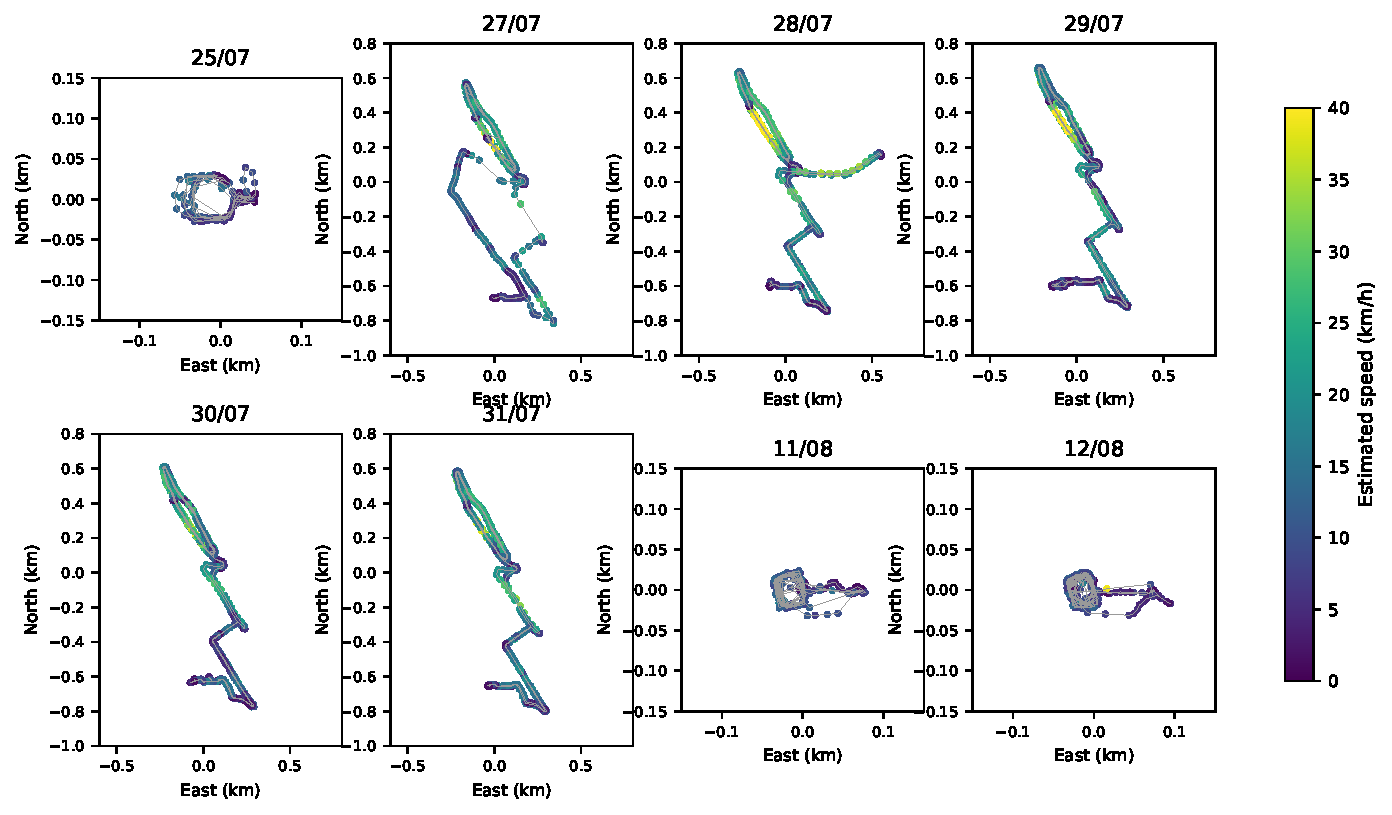
\includegraphics[width=\textwidth]{figuras/fig_9_geometria_rutas}
    \caption{Geometry of the eight sessions in relative local coordinates (not georeferenced), colored by estimated speed. The scales differ between the repeated route (27--31 July) and the confined circuits (25 July, 11 August, and 12 August).\label{fig:rutas}}
\end{figure}

The driving profile was derived from 2414 pairs of consecutive records separated by 4--6 s. Mean acceleration was $-0.006$ m/s$^2$, with a standard deviation of 0.24 m/s$^2$; the 5th and 95th percentiles were $-0.40$ and $+0.40$ m/s$^2$, and the maxima were $+0.85$ and $-1.75$ m/s$^2$. Acceleration ($>0.1$ m/s$^2$) accounted for 28.1\% of pairs, deceleration ($<-0.1$ m/s$^2$) for 29.2\%, and near-constant speed for 42.7\%; RPA was 0.10 m/s$^2$. Speed was below 10 km/h in 40.7\% of observations, between 10 and 20 km/h in 31.8\%, between 20 and 30 km/h in 22.0\%, and at least 30 km/h in 5.4\% (maximum, 49.2 km/h). The analysis identified 102 micro-trips with a median duration of 152.5 s (IQR, 75--215 s), a median distance of 326 m, and a mean speed of 9.8 km/h. A total of 161 gaps exceeded 30 s, including 111 longer than 60 s. Across records within the same session, 76.5\% of elapsed time fell within gaps longer than 30 s. Accordingly, the records describe movement rather than a complete stop-inclusive driving cycle (Figure~\ref{fig:perfil}). Acceleration levels were modest, consistent with a low-speed light vehicle, and should be compared with reference cycles only qualitatively \citep{ref-andre,ref-tutuianu,ref-brady}.

\begin{figure}[H]
    \centering
    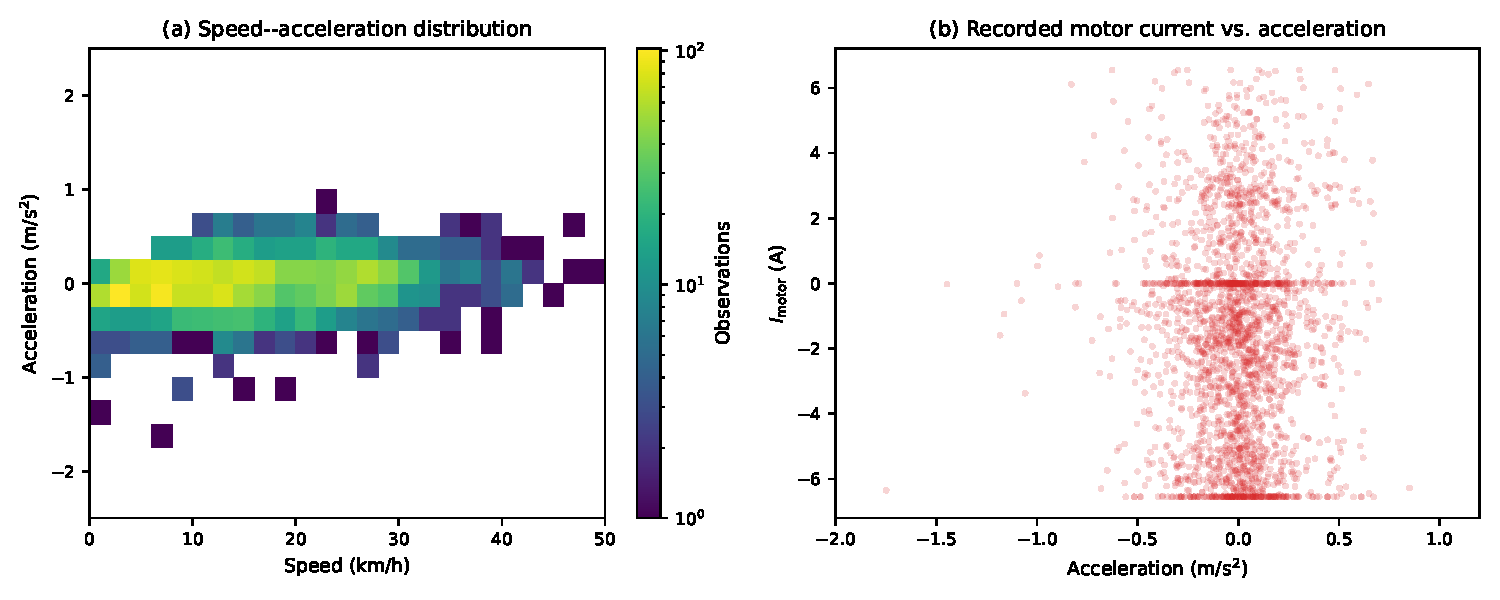
\includegraphics[width=0.95\textwidth]{figuras/fig_7_perfil_conduccion}
    \caption{Driving profile. (a) Joint distribution of speed and acceleration (2414 pairs of consecutive records). (b) Recorded motor current versus acceleration: no visible relationship is apparent, and the accumulation at $0$ and $\pm 6.55$ A indicates zero readings and saturation.\label{fig:perfil}}
\end{figure}

\subsection{Consistency of Speed with GPS Coordinates}\label{sec:gps}

The reported speed matched the value derived from the coordinates (2414 pairs): bias, $-1.6\times10^{-5}$ km/h; limits of agreement, $\pm 0.006$ km/h; RMSE, 0.0029 km/h; and correlation, 0.99999995. The difference is within the 0.01 km/h rounding precision, and the session RMSE ranged from 0.0028 to 0.0030 km/h. The reported incremental distance also matched the Haversine distance (RMSE, 0.0029 m). Thus, speed was calculated from the same GPS positions, and this comparison is a consistency check rather than an independent validation; it does not rule out GPS positioning or sampling errors \citep{ref-schuessler,ref-zandbergen}. Validation would require a wheel odometer or a reference GNSS receiver.

\subsection{Motor Current: Saturation, Baseline, and Response}

Recorded motor current was bounded at $\pm 6.55$ A (Figure~\ref{fig:potencia}). A total of 6.9\% of observations (210) coincided with this limit, almost all at the negative extreme (6.6\% versus 0.3\%), concentrated from 28 to 31 July (8.3--10.9\% per session; 0--0.5\% in the other sessions). Saturation was intermittent: 179 episodes were counted, with a median duration of 5 s (one observation) and a maximum of 15 s; only 4.3\% of saturated observations belonged to runs of three or more consecutive records. In addition, 9.4\% of observations had exactly zero current, and 18.1\% were within $\pm 0.5$ A. The 6.55 A limit is 14\% of the motor's maximum design current (46.3 A).

The current baseline varied between sessions (Table~\ref{tab:potencia}): mean current was $+0.38$ and $+0.90$ A on 25 and 27 July, ranged from $-1.78$ to $-2.23$ A from 28 to 31 July, and was $-1.11$ and $-1.52$ A in August. At speeds below 3 km/h ($n=362$), the median was $-1.40$ A (mean, $-2.03$ A). This offset represents a substantial fraction of the recorded range, and the shift between 27 and 28 July is consistent with a change in polarity, zero offset, or configuration between sessions; the data cannot determine which.

Recorded power had an absolute maximum of 357.5 W (17.9\% of the nominal 2 kW), a mean of $-72.8$ W, and 5th and 95th percentiles of $-314$ and $+188$ W. Its relationship with speed was negligible (Figure~\ref{fig:potencia}): $R^2=0.003$ for the regression of $|P|$ on speed (slope, 0.56 W per km/h; 95\% CI with 7 degrees of freedom, 0.08--1.04) and $R^2$ ranged from 0.001 to 0.066 across the eight sessions. Current also did not respond to acceleration: the pooled Spearman coefficient was $-0.01$ ($n=2414$), with session values from $-0.21$ to $+0.09$ (from $-0.06$ to $+0.18$ for $|I|$). Mean current was $-1.7$ A during weak deceleration and acceleration, $-1.1$ A during strong deceleration, and $-1.0$ A during strong acceleration (standard deviations, 3.1--3.5 A). A channel measuring traction current should show a clear dependence on acceleration. Excluding saturated observations did not change the result ($R^2=0.0004$).

\begin{table}[H]
    \caption{Recorded current and electrical power by session (signal indicators, not energy consumption). The 95\% CIs were obtained using a block bootstrap.\label{tab:potencia}}
    \small
    \setlength{\tabcolsep}{3pt}
    \begin{tabular}{l r r r r r}
        \toprule
        \textbf{Date} & \textbf{$n$} & \parbox{1.7cm}{\centering\textbf{Mean $I_{\mathrm{motor}}$                                                              \\(A)}} & \parbox{1.7cm}{\centering\textbf{Saturation\\(\%)}} & \parbox{2.9cm}{\centering\textbf{Mean $P$ (W)\\(95\% CI)}} & \parbox{2.9cm}{\centering\textbf{Gross energy\\(Wh/km; 95\% CI)}}\\
        \midrule
        25/07         & 114          & $+0.38$                                                    & 0.0  & 16.2 ($-$4.1; 66.0)          & 15.97 (13.90--18.95) \\
        27/07         & 369          & $+0.90$                                                    & 0.5  & 38.5 (13.3; 65.0)            & 6.37 (4.94--7.43)    \\
        28/07         & 448          & $-1.93$                                                    & 8.5  & $-$95.4 ($-$126.9; $-$78.2)  & 9.57 (7.29--12.27)   \\
        29/07         & 587          & $-1.78$                                                    & 8.3  & $-$88.0 ($-$118.8; $-$63.6)  & 12.75 (9.37--16.59)  \\
        30/07         & 638          & $-2.06$                                                    & 10.2 & $-$98.6 ($-$123.2; $-$62.4)  & 11.29 (8.53--13.91)  \\
        31/07         & 504          & $-2.23$                                                    & 10.9 & $-$107.3 ($-$128.7; $-$79.1) & 10.68 (8.77--12.09)  \\
        11/08         & 173          & $-1.11$                                                    & 0.0  & $-$57.3 ($-$102.5; $-$21.3)  & 16.32 (12.37--22.64) \\
        12/08         & 196          & $-1.52$                                                    & 0.5  & $-$77.9 ($-$117.9; $-$19.6)  & 20.69 (14.54--23.94) \\
        \bottomrule
    \end{tabular}
    \begin{flushleft}
        \footnotesize $P=V_{\mathrm{bat}}I_{\mathrm{motor}}$ using the channel sign. Gross energy integrates $|P|$ over intervals of up to 30 s and divides it by the distance covered during those intervals. Channel polarity is undocumented.
    \end{flushleft}
\end{table}

\begin{figure}[H]
    \centering
    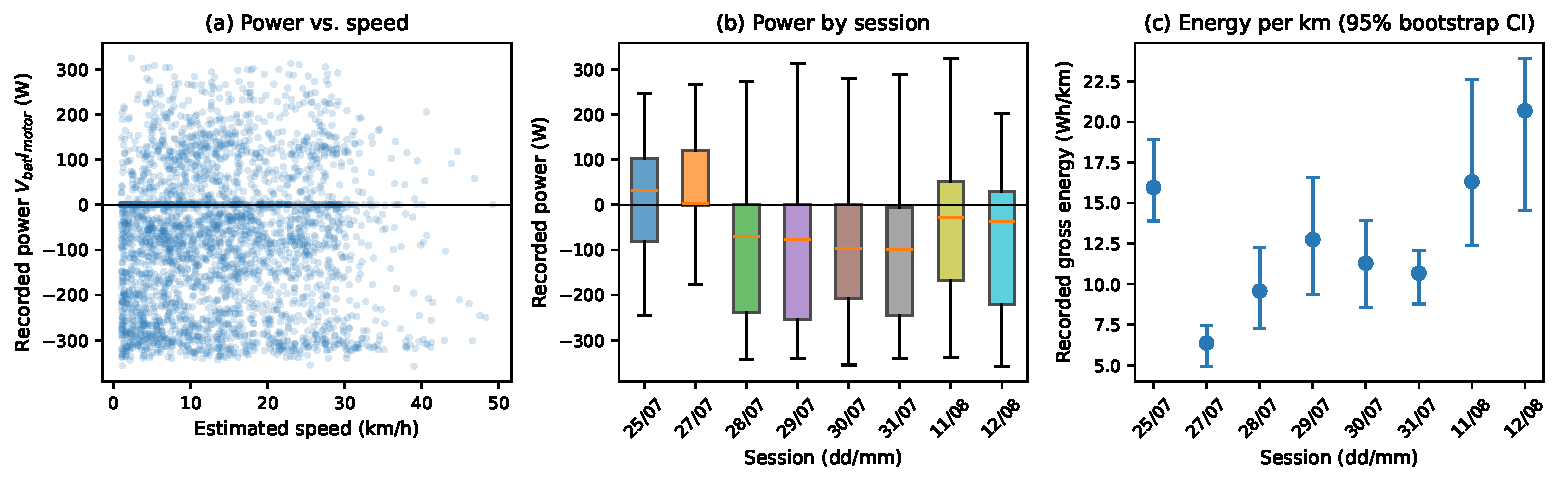
\includegraphics[width=\textwidth]{figuras/fig_5_potencia_energia}
    \caption{Recorded electrical power. (a) $V_{\mathrm{bat}}I_{\mathrm{motor}}$ versus estimated speed. (b) Distribution by session; the sign changes across dates. (c) Recorded gross energy per kilometer, with 95\% CIs from a block bootstrap. The limits at $\pm 320$ W in (a) correspond to current saturation.\label{fig:potencia}}
\end{figure}

The energy indicator depends more on processing decisions than on the routes. Mean gross energy across sessions was 12.96 Wh/km with a 30 s interval cap, but 11.6, 15.2, and 18.8 Wh/km with caps of 10, 60, and 120 s, respectively, and 13.0, 11.5, and 10.4 Wh/km with minimum speeds of 1, 3, and 5 km/h (Supplementary Table S5). This result, together with the dependence on polarity and zero offset, precludes interpreting the indicator as vehicle energy consumption.

\subsection{Panel Channel}

Across the eight analyzed sessions, current in the channel labeled as panel current was bounded at $\pm 3.28$ A: 14.0\% of observations were at this limit (13.97\% at $+3.28$ A), 34.4\% were exactly zero, and the median was 0.54 A (5th and 95th percentiles, $-0.92$ and $+3.28$ A). This limit is comparable to the converter's design current injected into the bus (3.51 A according to the specifications), but the data cannot determine whether it is a physical converter limit or a sensor limit. The channel was negatively correlated with motor current ($\rho=-0.45$), suggesting that the two channels are not independent or share a reference.

The known extreme values for this channel belong to the 21 July session, which is not among the eight analyzed sessions: the 18 retained observations from that date ranged from $-91.9$ to $68.0$ A (12 with $|I|>6.16$ A), and another 98 records from that day were excluded for exceeding 100 A; the maximum among the excluded records was 3200 A. These values are spurious for a circuit containing a 6.16 A module and lie outside the analyzed sessions.

Channel voltage ranged from 7.4 to 40.3 V, with a median of 30.0 V (Figure~\ref{fig:panel}a). In 87.3\% of observations, voltage was below the array's $V_{\mathrm{mp}}$ (34.2 V); 12.5\% fell between $V_{\mathrm{mp}}$ and $V_{\mathrm{oc}}$ (39.6 V), and only 0.2\% exceeded $V_{\mathrm{oc}}$. The voltage is compatible with a measurement at the converter input (range, 13--65 V), but this does not establish its origin. No time-of-day pattern was observed between 09:00 and 14:00: Spearman correlations with time were $-0.05$ for voltage and $-0.02$ for current (median session-level correlations, $-0.08$ and $0.01$, respectively), and hourly medians varied across sessions without a common trend (Figure~\ref{fig:panel}b). The lack of a pattern may reflect approximately constant irradiance during this window and does not demonstrate that the channel is insensitive to irradiance; without a pyranometer or reference cell, the signal cannot be associated with incident radiation.

\begin{figure}[H]
    \centering
    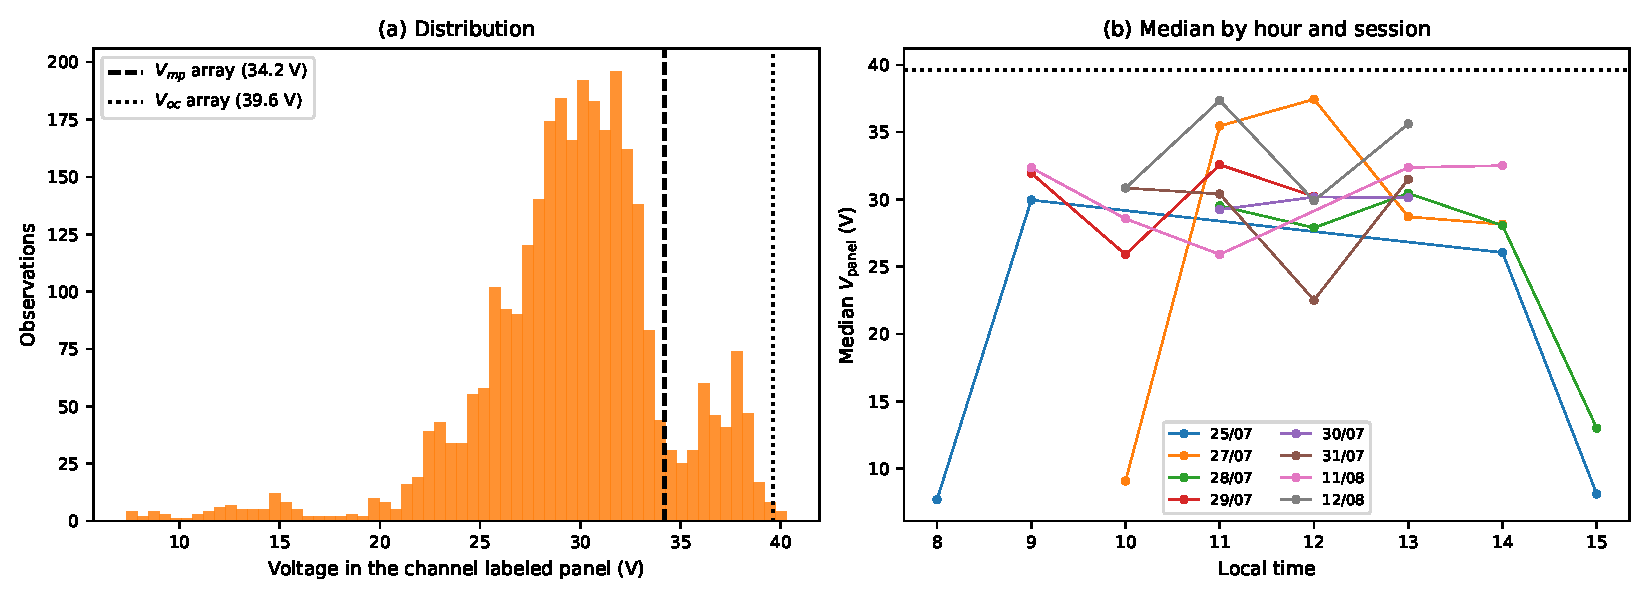
\includegraphics[width=\textwidth]{figuras/fig_8_canal_panel}
    \caption{Channel labeled as panel. (a) Voltage distribution relative to the array's documented $V_{\mathrm{mp}}$ and $V_{\mathrm{oc}}$. (b) Median voltage by local time and session.\label{fig:panel}}
\end{figure}

\subsection{Empirical Slope of Battery Voltage}

Battery voltage decreased as recorded motor current increased in all eight sessions, with an empirical slope $R_{\mathrm{ef}}$ of 0.15--0.73 $\Omega$ (mean, 0.30 $\Omega$; 95\% $t$-CI, 0.15--0.45; Supplementary Table S2). The pooled estimate with session fixed effects was 0.24 $\Omega$ (95\% CI with clustered errors and 7 degrees of freedom, 0.15--0.33; $R^2=0.15$). This slope is not an internal resistance: it is confounded by state of charge, temperature, and battery relaxation. Because controllers typically draw current depending on the available voltage, causality may operate in either direction. With eight sessions and current not exceeding 6.55 A, the result cannot be extrapolated to traction currents.

\subsection{Sensitivity of Results to Analytical Decisions}

The qualitative results are robust (Supplementary Table S5). The $R^2$ between speed and $|P|$ ranged from 0.0024 to 0.0028 for all minimum-coverage thresholds; saturation ranged from 6.9\% to 9.5\% (and from 7.3\% to 7.6\% with minimum speeds of 3 and 5 km/h); and maximum $|P|$ remained between 355 and 357 W. In contrast, integrated indicators depend on processing: with a minimum coverage of 200 records (five sessions), mean session speed increased from 12.5 to 15.2 km/h and gross energy decreased from 12.96 to 10.13 Wh/km. Doubling the block length from 30 to 60 increased the mean width of the speed CIs from 4.6 to 5.3 km/h.

\subsection{From Findings to Measurement Requirements}

Table~\ref{tab:hallazgos} summarizes the findings, the measurement failure they suggest, and the requirement that would address it. The failures are hypotheses about the measurement chain and should be verified through bench testing and system documentation.

\begin{table}[H]
    \caption{Findings, associated measurement failure, and requirement for the next campaign.\label{tab:hallazgos}}
    \footnotesize
    \setlength{\tabcolsep}{3pt}
    \renewcommand{\arraystretch}{1.1}
    \begin{tabular}{p{4.0cm} p{3.9cm} p{5.6cm}}
        \toprule
        \textbf{Finding} & \textbf{Suggested measurement failure}                                                                                                                                                       & \textbf{Requirement for the next campaign} \\
        \midrule
        $I_{\mathrm{motor}}$ bounded at $\pm 6.55$ A (6.9\%; 14\% of the 46.3 A design current)
                         & Insufficient sensor or converter range, or signal clipping
                         & Current sensor with a range of $\ge 60$ A (above the 57.9 A design current, including protection margin) and adequate resolution at cruising currents; verify using a calibrated clamp meter                                              \\
        Session-dependent $I_{\mathrm{motor}}$ baseline ($+0.9$ to $-2.2$ A); 9.4\% exact zeros
                         & Zero offset, polarity or configuration change; data loss recorded as zero
                         & Record zero with the vehicle stopped and circuit unloaded at the beginning and end of each session; document polarity and setup changes; encode missing data                                                                              \\
        $I_{\mathrm{motor}}$ does not depend on speed ($R^2=0.003$) or acceleration ($\rho=-0.01$)
                         & Channel does not measure total traction current
                         & Measure battery-bus and controller current using independent sensors and sampling at $\ge 1$ Hz                                                                                                                                           \\
        Panel channel: $\pm 3.28$ A, 34\% zeros, values from $-91.9$ to $68.0$ A on 21 July, and peaks up to 3200 A in excluded records
                         & Sensor or converter limit; defective scaling or connection
                         & Current and voltage sensors at the MPPT input and output, with documented measurement points and calibration before each campaign                                                                                                         \\
        No time-of-day pattern in $V_{\mathrm{panel}}$; no irradiance reference
                         & Missing synchronized environmental variable
                         & Pyranometer or reference cell in the module plane, module temperature, and battery state of charge, all with a common timestamp                                                                                                           \\
        Speed identical to the GPS-derived value (RMSE, 0.003 km/h); 76.5\% of elapsed time in gaps
                         & No independent speed reference; only movement is recorded
                         & Wheel odometer or reference GNSS; also record stops at uniform intervals                                                                                                                                                                  \\
        28.6\% of records excluded (46.7\% due to zero battery voltage)
                         & Acquisition or communication losses
                         & Record error codes rather than zeros; perform online quality control and retain raw-data copies                                                                                                                                           \\
        Specific energy ranges from 10.4 to 18.8 Wh/km depending on processing
                         & Irregular sampling and discontinuous records
                         & Continuous, uniform sampling to enable energy integration without interval caps                                                                                                                                                           \\
        \bottomrule
    \end{tabular}
\end{table}

\section{Discussion}

The data characterize prototype use: the repeated route and confined circuits differ in speed and geometry, and the driving profile features low acceleration and speeds predominantly below 20 km/h. Within- and between-session variability supports the view that a standardized cycle alone does not represent these usage patterns and that local cycles should be derived from local measurements \citep{ref-pfriem,ref-brady,ref-uberti}. However, prior movement-based filtering and gaps longer than 30 s prevent derivation of a complete driving cycle, daily distance, range, or energy consumption.

The electrical telemetry does not support common performance claims for a vehicle with integrated photovoltaics. Motor current is bounded, has an unstable baseline, and does not respond to speed or acceleration; the panel channel is also bounded, with approximately one-third of readings equal to zero. These signals do not demonstrate a solar contribution, and multiplying voltage by current without verified calibration, synchronization, sign convention, and measurement location does not yield metrologically defensible energy estimates \citep{ref-nist,ref-gum}. The sensitivity of integrated indicators to the interval cap reinforces this conclusion. The change in baseline before and after 27 July also suggests that setup changes should be documented as session metadata.

VIPV studies that quantify output while driving characterize irradiance and module electrical response \citep{ref-wetzel,ref-ng,ref-ota-irradiance,ref-ota-driving}; photovoltaic monitoring standards require defined variables and measurement points \citep{ref-iec61724}. In the present dataset, irradiance and module temperature were not recorded, and the current channels show fixed bounds and zero readings. Because the sensor locations, polarity, and calibration are undocumented, the underlying causes cannot be identified from these records alone. Table~\ref{tab:hallazgos} translates these measurement gaps into a minimum instrumentation protocol for future evaluations of solar contributions to traction. A standardized energy-consumption and range test \citep{ref-sae1634} would be meaningful only after the measurement chain has been verified.

\subsection{Limitations}

The study covers one vehicle, eight adequately covered sessions in July and August 2026, and two route types, with no controlled replicates; the findings therefore cannot be generalized to other vehicles, routes, or seasons. Sensor calibration and polarity, the actual measurement schematic, vehicle mass, and the algorithm used to calculate speed and distance are unavailable. Prior movement-based filtering and the exclusion criteria affect the analyzed dataset, and the 100-record threshold does not eliminate selection bias. The block-bootstrap CIs account for temporal dependence, but comparisons among only eight sessions remain indicative. Specific-energy indicators and the empirical slope depend on signals with unknown calibration. Gel-battery capacity and aging were not evaluated \citep{ref-ruetschi}, and irradiance, temperature, and state of charge were not measured. Consequently, the data support no conclusions about MPPT performance, solar contribution to traction, regenerative recovery, cost savings, or emissions reductions.

\section{Conclusions}

\begin{enumerate}
    \item Of 4277 movement records, 3052 records across 11 dates were retained; eight sessions (3029 records) supported between-session analysis. Zero battery-voltage readings accounted for 46.7\% of exclusions.
    \item Prototype use comprised a repeated route of approximately 1.4 km (mean speed, 14.7--16.0 km/h) and confined circuits (7.7--8.7 km/h), with moderate acceleration (5th and 95th percentiles: $\pm 0.40$ m/s$^2$) and speeds predominantly below 20 km/h.
    \item The reported speed is derived from GPS coordinates; no independent validation is available.
    \item Motor current is bounded at $\pm 6.55$ A, has a session-dependent baseline, and does not respond to speed or acceleration; the panel channel is bounded at $\pm 3.28$ A, with 34\% zero readings. The current measurement chain does not support estimates of energy consumption or photovoltaic generation.
    \item The observed measurement failures translate into specific instrumentation requirements: an appropriate current range, zero-offset and polarity verification, measurements at the MPPT input and output, synchronized irradiance, an independent speed reference, and continuous logging with error codes.
\end{enumerate}

\authorcontributions{Conceptualization, S.P; methodology, C.C.; software, C.C.; validation, S.P., M.S. and P.P.; formal analysis, P.P.; investigation, M.S.; resources, S.P.; data curation, C.C.; writing---original draft preparation, M.S.; writing---review and editing, S.P.; supervision, P.P.; project administration, S.P.; funding acquisition, S.P. All authors have read and agreed to the published version of the manuscript.}
\funding{This work was supported by the Instituto Tecnológico Superior Rumiñahui (ISTER) through its research department.}
\dataavailability{The data used in this manuscript are available at \url{https://github.com/MaxwellSalazar/vehicle_electric.git}.}
\acknowledgments{The prototype was developed and field-tested with institutional and financial support from the Instituto Tecnológico Superior Rumiñahui (ISTER). The authors thank the researchers, students, and administrative staff who contributed to vehicle design, data collection, and field testing in Sangolquí.}
\conflictsofinterest{The authors declared no potential conflicts of interest with respect to the research, authorship, and/or publication of this article.}

\section*{Abbreviations}
\noindent
BLDC: brushless direct current; GNSS: Global Navigation Satellite System; GPS: Global Positioning System; CI: confidence interval; MAD: median absolute deviation; MPPT: maximum power point tracking; IQR: interquartile range; RPA: relative positive acceleration; VIPV: vehicle-integrated photovoltaics; VRLA: valve-regulated lead-acid; Wp: watt-peak.

\reftitle{References}
\begin{thebibliography}{999}
    \bibitem[Commault et al.(2021)]{ref-commault}
    Commault, B.; Duigou, T.; Maneval, V.; Gaume, J.; Chabuel, F.; Voroshazi, E. Overview and Perspectives for Vehicle-Integrated Photovoltaics. \textit{Applied Sciences} \textbf{2021}, \textit{11}, 11598. https://doi.org/10.3390/app112411598.

    \bibitem[Sierra Rodriguez et al.(2020)]{ref-sierra}
    Sierra Rodriguez, A.; de Santana, T.; MacGill, I.; Ekins-Daukes, N.J.; Reinders, A. A feasibility study of solar PV-powered electric cars using an interdisciplinary modeling approach for the electricity balance, CO$_2$ emissions, and economic aspects: The cases of The Netherlands, Norway, Brazil, and Australia. \textit{Progress in Photovoltaics: Research and Applications} \textbf{2020}, \textit{28}, 517--532. https://doi.org/10.1002/pip.3202.

    \bibitem[Hoth et al.(2024)]{ref-hoth}
    Hoth, P.; Heide, L.; Grahle, A.; Göhlich, D. Vehicle-Integrated Photovoltaics---A Case Study for Berlin. \textit{World Electric Vehicle Journal} \textbf{2024}, \textit{15}, 113. https://doi.org/10.3390/wevj15030113.

    \bibitem[Kouzelis et al.(2025)]{ref-kouzelis}
    Kouzelis, A.; Linders, K.; Bandyopadhyay, S.; Mouli, G.R.C. Analysis of vehicle-integrated photovoltaics and vehicle-to-grid on electric vehicle battery life. \textit{Journal of Power Sources} \textbf{2025}, \textit{631}, 236117. https://doi.org/10.1016/j.jpowsour.2024.236117.

    \bibitem[Wetzel et al.(2022)]{ref-wetzel}
    Wetzel, G.; Salomon, L.; Krügener, J.; Bredemeier, D.; Peibst, R. High time resolution measurement of solar irradiance onto driving car body for vehicle integrated photovoltaics. \textit{Progress in Photovoltaics: Research and Applications} \textbf{2022}, \textit{30}, 543--551. https://doi.org/10.1002/pip.3526.

    \bibitem[Ng et al.(2020)]{ref-ng}
    Ng, C.W.X.; Zhang, J.; Tay, S.E.R. A Tropical Case Study Quantifying Solar Irradiance Collected on a Car Roof for Vehicle Integrated Photovoltaics Towards Low-Carbon Cities. In \textit{Proceedings of the 2020 47th IEEE Photovoltaic Specialists Conference (PVSC)}, Calgary, AB, Canada, 15--21 June 2020; pp. 2461--2464. https://doi.org/10.1109/PVSC45281.2020.9300351.

    \bibitem[Ota et al.(2019)]{ref-ota-irradiance}
    Ota, Y.; Masuda, T.; Araki, K.; Yamaguchi, M. A mobile multipyranometer array for the assessment of solar irradiance incident on a photovoltaic-powered vehicle. \textit{Solar Energy} \textbf{2019}, \textit{184}, 84--90. https://doi.org/10.1016/j.solener.2019.03.084.

    \bibitem[Ota et al.(2021)]{ref-ota-driving}
    Ota, Y.; Araki, K.; Nagaoka, A.; Nishioka, K. Evaluating the output of a car-mounted photovoltaic module under driving conditions. \textit{IEEE Journal of Photovoltaics} \textbf{2021}, \textit{11}, 1299--1304. https://doi.org/10.1109/JPHOTOV.2021.3087748.

    \bibitem[Ota et al.(2022)]{ref-ota-curve}
    Ota, Y.; Araki, K.; Nagaoka, A.; Nishioka, K. Curve correction of vehicle-integrated photovoltaics using statistics on commercial car bodies. \textit{Progress in Photovoltaics: Research and Applications} \textbf{2022}, \textit{30}, 152--163. https://doi.org/10.1002/pip.3473.

    \bibitem[Bhavsar et al.(2024)]{ref-bhavsar}
    Bhavsar, D.; Jaychandra, R.K.; Mittal, M. Data acquisition and performance analysis during real-time driving of a two-wheeler electric vehicle---A case study. \textit{World Electric Vehicle Journal} \textbf{2024}, \textit{15}, 121. https://doi.org/10.3390/wevj15030121.

    \bibitem[Al-Wreikat et al.(2021)]{ref-alwreikat}
    Al-Wreikat, Y.; Serrano, C.; Sodré, J.R. Driving behaviour and trip condition effects on the energy consumption of an electric vehicle under real-world driving. \textit{Applied Energy} \textbf{2021}, \textit{297}, 117096. https://doi.org/10.1016/j.apenergy.2021.117096.

    \bibitem[Pfriem and Gauterin(2016)]{ref-pfriem}
    Pfriem, M.; Gauterin, F. Development of real-world driving cycles for battery electric vehicles. \textit{World Electric Vehicle Journal} \textbf{2016}, \textit{8}, 14--24. https://doi.org/10.3390/wevj8010014.

    \bibitem[Brady and O'Mahony(2016)]{ref-brady}
    Brady, J.; O'Mahony, M. Development of a driving cycle to evaluate the energy economy of electric vehicles in urban areas. \textit{Applied Energy} \textbf{2016}, \textit{177}, 165--178. https://doi.org/10.1016/j.apenergy.2016.05.094.

    \bibitem[Uberti et al.(2020)]{ref-uberti}
    Uberti, S.; Azzini, G.; Beltrami, D.; Tribioli, L.; Iora, P. Modelling of a 15-kW electric utility vehicle and range assessment through driving cycle analysis based on GPS experimental data. SAE Technical Paper 2020-24-0018, 2020. https://doi.org/10.4271/2020-24-0018.

    \bibitem[Künsch(1989)]{ref-kunsch}
    Künsch, H.R. The Jackknife and the Bootstrap for General Stationary Observations. \textit{The Annals of Statistics} \textbf{1989}, \textit{17}, 1217--1241. https://doi.org/10.1214/aos/1176347265.

    \bibitem[Cliff(1993)]{ref-cliff}
    Cliff, N. Dominance Statistics: Ordinal Analyses to Answer Ordinal Questions. \textit{Psychological Bulletin} \textbf{1993}, \textit{114}, 494--509. https://doi.org/10.1037/0033-2909.114.3.494.

    \bibitem[Virtanen et al.(2020)]{ref-scipy}
    Virtanen, P.; Gommers, R.; Oliphant, T.E.; et al. SciPy 1.0: Fundamental Algorithms for Scientific Computing in Python. \textit{Nature Methods} \textbf{2020}, \textit{17}, 261--272. https://doi.org/10.1038/s41592-019-0686-2.

    \bibitem[Seabold and Perktold(2010)]{ref-statsmodels}
    Seabold, S.; Perktold, J. statsmodels: Econometric and Statistical Modeling with Python. In Proceedings of the 9th Python in Science Conference, Austin, TX, USA, 28 June--3 July 2010; pp. 92--96. https://doi.org/10.25080/Majora-92bf1922-011.

    \bibitem[Taylor and Kuyatt(1994)]{ref-nist}
    Taylor, B.N.; Kuyatt, C.E. \textit{Guidelines for Evaluating and Expressing the Uncertainty of NIST Measurement Results}; NIST Technical Note 1297; National Institute of Standards and Technology: Gaithersburg, MD, USA, 1994. https://doi.org/10.6028/NIST.TN.1297.

    \bibitem[JCGM(2008)]{ref-gum}
    Joint Committee for Guides in Metrology (JCGM). \textit{Evaluation of Measurement Data---Guide to the Expression of Uncertainty in Measurement}; JCGM 100:2008; BIPM: Sèvres, France, 2008. https://doi.org/10.59161/JCGM100-2008E.

    \bibitem[IEC(2021)]{ref-iec61724}
    International Electrotechnical Commission (IEC). \textit{IEC 61724-1:2021: Photovoltaic System Performance---Part 1: Monitoring}; IEC: Geneva, Switzerland, 2021. Available online: \url{https://webstore.iec.ch/en/products}.

    \bibitem[SAE International(2021)]{ref-sae1634}
    SAE International. \textit{SAE J1634\_202104: Electric Vehicle Energy Consumption and Range Test Procedure}; SAE International: Warrendale, PA, USA, 2021. Available online: \url{https://www.sae.org/standards/content/j1634_202104/}.

    \bibitem[Ruetschi(2004)]{ref-ruetschi}
    Ruetschi, P. Aging mechanisms and service life of lead--acid batteries. \textit{Journal of Power Sources} \textbf{2004}, \textit{127}, 33--44. https://doi.org/10.1016/j.jpowsour.2003.09.052.

    \bibitem[André et al.(2004)]{ref-andre}
    André, M. The ARTEMIS European driving cycles for measuring car pollutant emissions. \textit{Science of the Total Environment} \textbf{2004}, \textit{334--335}, 73--84. https://doi.org/10.1016/j.scitotenv.2004.04.070.

    \bibitem[Schuessler and Axhausen(2009)]{ref-schuessler}
    Schuessler, N.; Axhausen, K.W. Processing Raw Data from Global Positioning Systems without Additional Information. \textit{Transportation Research Record} \textbf{2009}, \textit{2105}, 28--36. https://doi.org/10.3141/2105-04.

    \bibitem[Tutuianu et al.(2015)]{ref-tutuianu}
    Tutuianu, M.; Bonnel, P.; Ciuffo, B.; Haniu, T.; Ichikawa, N.; Marotta, A.; Pavlovic, J.; Steven, H. Development of the World-wide harmonized Light duty Test Cycle (WLTC) and a possible pathway for its introduction in the European legislation. \textit{Transportation Research Part D} \textbf{2015}, \textit{40}, 61--75. https://doi.org/10.1016/j.trd.2015.07.011.

    \bibitem[Zandbergen(2009)]{ref-zandbergen}
    Zandbergen, P.A. Accuracy of iPhone Locations: A Comparison of Assisted GPS, WiFi and Cellular Positioning. \textit{Transactions in GIS} \textbf{2009}, \textit{13}, 5--25. https://doi.org/10.1111/j.1467-9671.2009.01152.x.

    \bibitem[Hu et al.(2022)]{ref-hu}
    Hu, C.; Li, B.; Ma, L.; Cheng, F. State-of-charge estimation for lithium-ion batteries of electric vehicle based on sensor random error compensation. \textit{Journal of Energy Storage} \textbf{2022}, \textit{55}, 105537. https://doi.org/10.1016/j.est.2022.105537.

    \bibitem[Zheng et al.(2020)]{ref-zheng}
    Zheng, C.; Chen, Z.; Huang, D. Fault diagnosis of voltage sensor and current sensor for lithium-ion battery pack using hybrid system modeling and unscented particle filter. \textit{Energy} \textbf{2020}, \textit{191}, 116504. https://doi.org/10.1016/j.energy.2019.116504.

    \bibitem[Gurusamy and Ashok(2024)]{ref-gurusamy}
    Gurusamy, A.; Ashok, B. Establishment of electric two-wheeler driving cycle for energy economy and life cycle assessment under Indian Tier-2 city driving environments. \textit{Sustainable Energy Technologies and Assessments} \textbf{2024}, \textit{66}, 103826. https://doi.org/10.1016/j.seta.2024.103826.
\end{thebibliography}
\end{document}
